\documentclass[12pt, a4paper]{article}

\usepackage{graphicx}
\graphicspath{{figures/}}

\usepackage{subcaption}

\usepackage{float}

\usepackage{wrapfig}

\usepackage{amsmath}

\title{My first document}
\author{gendloop\thanks{gg}}
\date{July 2024}

\begin{document}

\maketitle
You have now added a title, author and date to your first \LaTeX{} document
Hello gendloop, this is your first document.
This is a simple example, with no extra parameters or packages included.

% comment

Bold: \textbf{Bold}
Italics: \textit{Italics}
Underline: \underline{Underline}

% \emph
Some of the greatest \emph{discoveries} in science were made by accident

\textit{Some of the greatest \emph{discoveries} in science were made by accident}

\textbf{Some of the greatest \emph{discoveries} in science were made by accident}

% -- Adding images --

% example 1

\includegraphics{favicon.png}

% example 2
\begin{figure}[H]
    \centering
    
\includegraphics[width=0.1\textwidth]{favicon.png}
    \caption{A nice picture}
    \label{fig:mesh1}
\end{figure}

\begin{figure}[H]
    \centering
    
\includegraphics[width=0.1\textwidth]{favicon.png}
    \caption{A nice picture 2}
    \label{fig:mesh2}
\end{figure}

% example 3
As you can see in figure \ref{fig:mesh1}, the function grows near the origin.
This example is on page \pageref{fig:mesh1}.

% example 4: Multiple images in one figure
\begin{figure}[H]
    \centering
    \begin{subfigure}{0.4\textwidth}
        
\includegraphics[width=\linewidth]{favicon.png}
        \caption{Caption1}
        \label{fig:subimg1}
    \end{subfigure}
    \begin{subfigure}{0.4\textwidth}
        
\includegraphics[width=\linewidth]{favicon.png}
        \caption{Caption2}
        \label{fig:subimg2}
    \end{subfigure}

    \caption{Caption for this figure with two images}
    \label{fig:img2}
\end{figure}

% example 5: Chanaging the image size and rotating the picture

\includegraphics[scale=0.1]{favicon.png}

\includegraphics[scale=0.2]{favicon.png}

\includegraphics[scale=0.3]{favicon.png}

\includegraphics[width=4cm, height=2cm]{favicon.png}

\includegraphics[scale=0.2, angle=45]{favicon.png}

% example 6: Wrapping text around figures
Praesent in sapien. Lorem ipsum dolor sit amet, consectetuer
adipiscing elit. Duis fringilla tristique neque. Sed interdum
libero ut metus. Pellentesque placerat.

\begin{wrapfigure}{l}{0.25\textwidth} % r,l,i,o
    \centering
    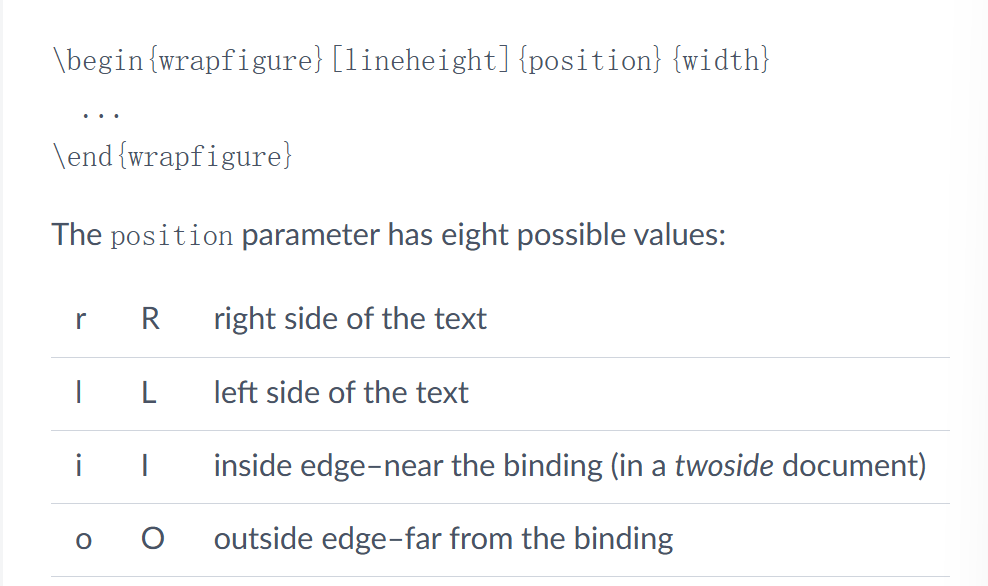
\includegraphics[width=\linewidth]{wrap_figure.png}
\end{wrapfigure}

Praesent in sapien. Lorem ipsum dolor sit amet, consectetuer
adipiscing elit. Duis fringilla tristique neque. Sed interdum
libero ut metus. Pellentesque placerat.

% -- Creating lists --

% Unordered lists
\begin{itemize}
    \item apple
    \item banana
\end{itemize}

% ordered lists
\begin{enumerate}
    \item apple
    \item banana
\end{enumerate}

% mixed
\begin{enumerate}
    \item first
    \begin{itemize}
        \item apple
        \item pear
    \end{itemize}
    \item second
    \begin{enumerate}
        \item apple
        \item pear
    \end{enumerate}
\end{enumerate}

% -- math --

% Inline math mode
In physics, the mass-energy equivalence is stated
by the wquation $E=mc^2$, discovered in 1905 by Albert Einstein.

\(E=mc^2\)

$E=mc^2$

\begin{math}
    E=mc^2
\end{math}

% Display math mode
In physics, the mass-energy equivalence is stated
by the wquation \[E=mc^2\], discovered in 1905 by Albert Einstein.

\begin{equation}
    E=m^2 % 带序号
\end{equation}

\begin{equation*}
    E=m^2 % 带序号
\end{equation*}

% Complete example
Subscripts in math mode are written as $a_b$ and superscripts are written as $a^b$. These can be combined and nested to write expressions such as

\[ T^{i_1 i_2 \dots i_p}_{j_1 j_2 \dots j_q} = T(x^{i_1},\dots,x^{i_p},e_{j_1},\dots,e_{j_q}) \]

We write integrals using $\int$ and fractions using $\frac{a}{b}$. Limits are placed on integrals using superscripts and subscripts:

\[ \int_0^1 \frac{dx}{e^x} =  \frac{e-1}{e} \]

Lower case Greek letters are written as $\omega$ $\delta$ etc. while upper case Greek letters are written as $\Omega$ $\Delta$.

Mathematical operators are prefixed with a backslash as $\sin(\beta)$, $\cos(\alpha)$, $\log(x)$ etc.

\end{document}
